\section{Tabelle e grafici}
Here a few examples of tables and graphs.
\subsection{Tabelle}
\begin{center}
\begin{tabular}{c c c c c c c c}
\arrayrulecolor{Azzurro}
\hline
{\bfseries $Codice$} & {\bfseries $CdL$} & {\bfseries $Lotto$} & {\bfseries $T_{setup/lotto}$} & {\bfseries $T_{lav/pezzo}$} & {\bfseries $T_{proc/pezzo}$} & {\bfseries$Quantit\grave{a}$} & {\bfseries $T_{tot}$}\\
\hline
100 & 4 & 250 & 25 & 0,5 & 0,6 & 1 & 0,6\\
111 & 2 & 250 & 20 & 2 & 2,08 & 1 & 2,08 \\
111 & 3 & 250 & 15 & 1,5 & 1,56 & 1 & 1,56 \\
112 & 2 & 250 & 20 & 2,5 & 2,58 & 1 & 2,58 \\
112 & 3 & 250 & 15 & 2 & 2,06 & 1 & 2,06\\
113 & 3 & 500 & 15 & 1 & 1,03 & 2 & 2,06\\
120 & 1 & 50 & 30 & 2 & 2,6 & 0,1 & 0,26\\
121 & 1 & 25 & 30 & 3 & 4,2 & 0,1 & 0,42 \\
121 & 1 & 25 & 30 & 2,5 & 3,7 & 0,1 & 0,37 \\
\hline
\end{tabular}
\end{center}

\subsubsection{Altra tabella}
\begin{center}
\begin{tabular}{l c c c c c c c c c}
\arrayrulecolor{Azzurro}
\hline
{\bfseries Periodo} & 1 & 2 & 3 & 4 & 5 & 6 & 7 & 8 & Media\\
\hline
{\bfseries MPS} & 250 & 250 & 250 & 250 & 250 & 250 & 250 & 250 & \\
{\bfseries CdL 1} & 262,5 & 262,5 & 262,5 & 262,5 & 262,5 & 262,5 & 262,5 & 262,5 & 262,5\\
{\bfseries CdL 2} & 1165 & 1165 & 1165 & 1165 & 1165 & 1165 & 1165 & 1165 & 1165\\
{\bfseries CdL 3} & 1420 & 1420 & 1420 & 1420 & 1420 & 1420 & 1420 & 1420 & 1420\\
{\bfseries CdL 4} & 150 & 150 & 150 & 150 & 150 & 150 & 150 & 150 & 150\\
\hline
\end{tabular}
\end{center}

\subsection{Grafici}
\begin{center}
\begin{figure}[H]
\begin{tikzpicture}
\begin{axis}[
/pgf/number format/.cd,
        use comma,
        1000 sep={},
ybar,
ymin=0,ymax=2000,
ymajorgrids=true,
ylabel=,
xlabel=,
major x tick style = transparent,
enlarge x limits=0.1,
legend style={draw=none,font=\scriptsize,cells={anchor=west}},
symbolic x coords={1,2,3,4,5,6,7,8},
bar width=5pt, %!!!!!!!!!!!!!!!!
xtick=data,
nodes near coords={
    \rotatebox{90}{%
    \tiny
    \pgfmathprintnumber[fixed,precision=0,zerofill]\pgfplotspointmeta
    }
},
nodes near coords align={vertical},
width=13cm,
height=8cm,
legend style={
    legend pos=outer north east,
    legend columns=1,
}
]
\addplot[draw=Rosso, fill=Rosso] coordinates    {(1,262.5) (2,262.5) (3,262.5) (4,262.5) (5,262.5) (6,262.5) (7,262.5) (8,262.5)};    
\addplot [draw=Viola, fill=Viola] coordinates
    {(1,1165) (2,1165) (3,1165) (4,1165) (5,1165) (6,1165) (7,1165) (8,1165)};    
\addplot [draw=Arancione, fill=Arancione] coordinates
    {(1,1420) (2,1420) (3,1420) (4,1420) (5,1420) (6,1420) (7,1420) (8,1420)};    
    \addplot [draw=Celeste, fill=Celeste] coordinates
    {(1,150) (2,150) (3,150) (4,150) (5,150) (6,150) (7,150) (8,150)}; 

\legend{CdL 1, CdL 2, CdL 3, CdL 4}
\end{axis}
\end{tikzpicture}
\end{figure}
\end{center}

\subsubsection{Altro grafico}
\begin{center}


\begin{tikzpicture}

    
        
    \draw[->,name path=xaxis] (-0.2,0) -- (10.2,0) node[right] {$t$};
    \draw[->,name path=yaxis] (0,-0.8) -- (0,3.2) node[above] {Livello $x(t)$};

    % lines  
    \draw[name path=line1,domain=0:5] plot (\x,{2-2/3* \x}) node[above right] {};
    \draw[name path=line2,domain=-0.666:2] plot ({4},\x) node[below right] {};
    \draw[name path=line3,domain=4:8] plot (\x,{14/3-2/3* \x}) node[above right] {};
    \draw[name path=line4,domain=0:9,  draw=gray] plot (\x,{2}) node[above right] {};
    \draw[name path=line5,domain=0:9,  draw=gray] plot (\x,{-0.666}) node[above right] {};
\draw[name path=line6,domain=0:-1.7,  draw=gray] plot ({0}, \x) node[above right] {};
    \draw[name path=line7,domain=0:-1.7,  draw=gray] plot ({4},\x) node[above right] {};
    \draw[name path=line8,domain=0:-1.1,  draw=gray] plot ({3},\x) node[above right] {};
    
    % calculate intersection points
    \node[name intersections={of=line1 and line2}] (a) at (intersection-1)  {};
    \node[name intersections={of=line2 and line3}] (b) at (intersection-1) {};
    \node[name intersections={of=line1 and xaxis}] (c) at (intersection-1) {};
    \node (d) at (0,0) {};
    \node[name intersections={of=yaxis and line1}] (e)  at (intersection-1){};
    \node[name intersections={of=line2 and xaxis}] (f) at (intersection-1) {};
    \node[name intersections={of=line3 and xaxis}] (g) at (intersection-1) {};
    
    % draw the big polygon    
    \filldraw[fill=Azzurro,fill opacity=0.4] (c.center) -- (d.center) -- (e.center) -- cycle;
\filldraw[fill=Blu,fill opacity=0.7] (f.center) -- (a.center) -- (c.center) -- cycle;
   \filldraw[fill=Azzurro,fill opacity=0.4] (g.center) -- (f.center) -- (b.center) -- cycle; 
   
  \draw [<->] (9,1.9) -- (9,-0.566); 
  \node[align=left, right] at (9,0.667) {$Q$}; 
  \draw [<->] (8.2,-0.1) -- (8.2,-0.566); 
  \node[align=left, right] at (8.2,-0.333) {$B$};
  
  \draw [<->] (0.1,-1.7) -- (3.9,-1.7); 
  \node[] at (2,-1.95) {$T$};
  \draw [<->] (0.1,-1.1) -- (2.9,-1.1); 
  \node[] at (1.5,-1.35) {$t_{i}$};
  \draw [<->] (3.1,-1.1) -- (3.9,-1.1); 
  \node[] at (3.5,-1.35) {$t_{b}$};
  
 \draw [] (4.872,-0.666) arc [start angle=0, end angle=-30, radius=1cm]
    node [midway, right] {$r$};   
 
\end{tikzpicture}
\end{center}
\newpage

\section{Formule}
Se non sono ammesse consegne in ritardo siamo in presenza di un problema con Backlog. Sia $ t_{i} $ il periodo in cui non si è in backlog e $ t_{b} $ il periodo di backlog. Essendo $ t_{i}=(Q-B)/D $, avremo:\\
Costi di ordinazione = $C\cdot D/Q$\\
Costi di mantenimento = $ H\cdot (Q-B)/2\cdot t_{i}/T=H\cdot (Q-B)^{2}/2Q $\\
Costi di backorder = $ C_{b}\cdot B\cdot t_{b}/2T=C_{b}\cdot B^{2}/2Q $\\
Costi variabili totali = $ TC(Q)=C\cdot D/Q+H\cdot (Q-B)^{2}/2Q+C_{b}\cdot B^{2}/2Q $\\
Condizioni di minimo: 
$\begin{cases}
\frac{\partial TC}{\partial Q}=0\\\frac{\partial TC}{\partial B}=0
\end{cases}
\Rightarrow
Q^{\ast}=\sqrt{\dfrac{2C\cdot D(H+C_{b})}{H\cdot C_{b}}}=EOQ\sqrt{\dfrac{H+C_{b}}{C_{b}}}
$

\section{Altro}
\begin{figure}[H]
\centering
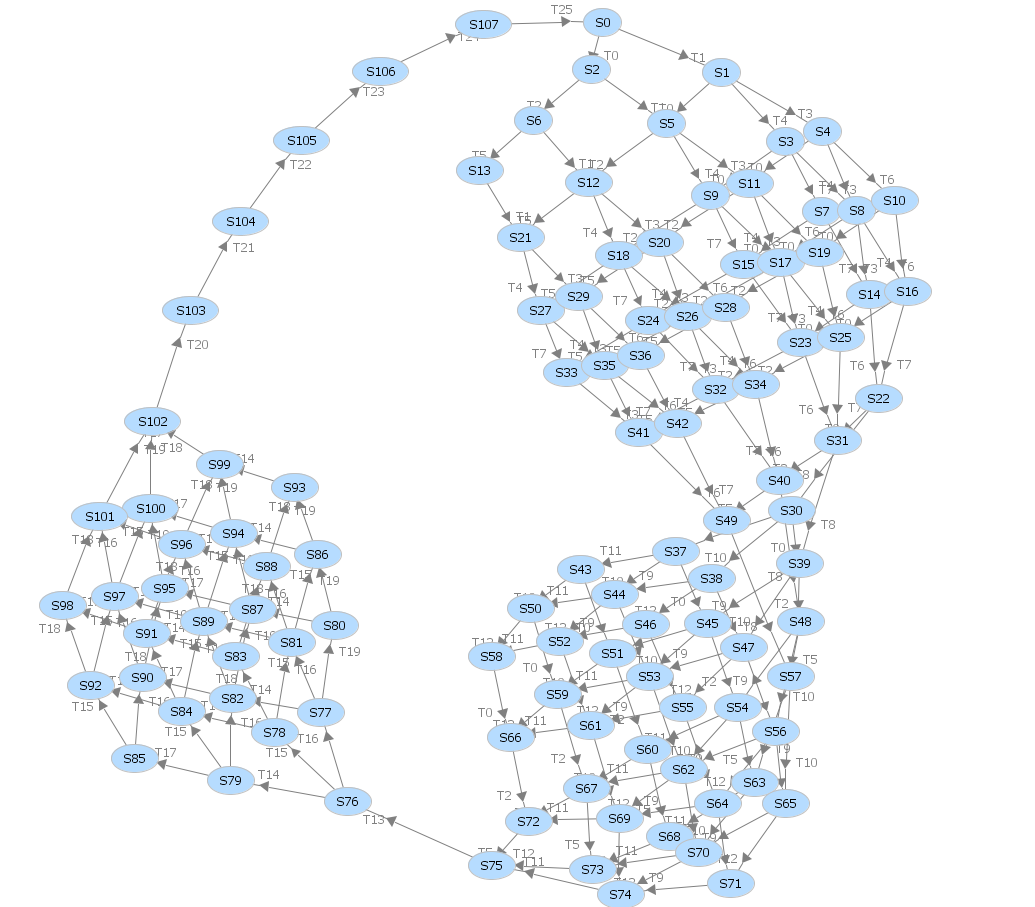
\includegraphics[width=1\textwidth]{grafo.png}
\caption{\label{fig:1}Didascalia.}
\end{figure}
\subsection{Footnote}
You can create a footnote like this.\footnote{I created a footnote.}

\subsection{Flowchart}
\newpage
\begin{landscape}
\thispagestyle{empty}
\singlespacing
\noindent
\begin{tikzpicture}[overlay,remember picture,node distance = 3.5cm, auto]
\coordinate (0) at (current page.north);
\tikzstyle{decision} = [diamond,aspect=2, draw=Blu,line width=0.6mm, fill=Blu!10, minimum height=1em,
    text width=6em, text badly centered,  inner sep=0pt]
\tikzstyle{block} = [rectangle, draw=Blu,line width=0.6mm, fill=white, text width=5em, text badly centered, rounded corners, minimum height=1em]
\tikzstyle{line} = [draw, -latex']
\tikzstyle{cloud} = [draw=white, ellipse,fill=Blu, node distance=1.5cm,
    minimum height=2em]
    
    % Place nodes
    
    \node [decision][shift={(19.5 cm,-8cm)}]  at (current page.north) (init) {\scriptsize Prodotto standard?};
    \node [cloud, above of=init] (system) {\scriptsize\textcolor{white}{Ricezione ordine dal cliente}};
    \node [decision, right of=init,node distance=4.5cm] (registrosi) {\scriptsize Il cliente accetta di ordinare almeno un cartone di prodotto?};
    \node [decision, right of=registrosi,node distance=4.8cm] (100) {\scriptsize Cambia prodotto?};
    \node [block, right of=100,node distance=3.5cm] (101) {\scriptsize Ciao!};
    \node [decision, below of=init, node distance=2cm] (identify) {\scriptsize  Nuovo cliente?};
    \node [block, below of=identify, node distance=1.7cm] (102) {\scriptsize  Compilo foglio di lavoro};
    \node [block, below of=102, node distance=1.7cm] (103) {\scriptsize  L'operatore prende il foglio di lavoro};
    \node [block, below of=103, node distance=1.9cm] (104) {\scriptsize  Va in magazzino e prende le scatole necessarie};
   \node [decision, below of=104, node distance=2.2cm] (105) {\scriptsize  Le scatole sono rovinate?};
   \node [block, below of=105, node distance=2.4cm] (106) {\scriptsize  Metto le scatole nel cartone per l'imballaggio}; 
   \node [decision, below of=106, node distance=2.2cm] (107) {\scriptsize  Manca qualche articolo?};
   \node [block, right of=107, node distance=4.5cm] (108) {\scriptsize  Sposto il cartone in zona di attesa};
   \node [block, above of=108, node distance=1.5cm] (109) {\scriptsize  Riporto il foglio di lavoro in ufficio};
   \node [block, above of=109, node distance=3.5cm] (110) {\scriptsize  Contatto cliente e avviso sui nuovi tempi di consegna};
   \node [decision, right of=110, node distance=4cm] (111) {\scriptsize  Il cliente è disponibile all'attesa?};
   \node [block, right of=111, node distance=4cm] (112) {\scriptsize  Propongo articolo similare disponibile in magazzino};
   \node [decision, above of=112, node distance=2.5cm] (113) {\scriptsize  Va bene?};
   \node [decision, above of=113, node distance=2.7cm] (114) {\scriptsize  Il cliente vuole comunque gli altri articoli?};
   \node [block, above of=114, node distance=2.2cm] (115) {\scriptsize  Aggiorno il foglio di lavoro};
   \node [block, left of=114, node distance=4.5cm] (116) {\scriptsize  Annullo ordine};
   \node [block, below of=111, node distance=2.3cm] (117) {\scriptsize  Contatto fornitore e ordino gli articoli mancanti};
   \node [block, below of=117, node distance=1.5cm] (118) {\scriptsize  Arrivo merce};
   \node [block, below of=118, node distance=1.3cm] (119) {\scriptsize  Smisto in magazzino};
   \node [block, below of=119, node distance=2cm] (120) {\scriptsize  Aggiungo gli astucci mancanti nel cartone per l'imballaggio};
   \node [block, right of=118, node distance=6cm] (121) {\scriptsize  Aggiorno il foglio di lavoro};
   \node [block, left of=identify, node distance=3.5cm] (122) {\scriptsize  Registro anagrafica cliente};
   \node [decision, left of=122, node distance=4cm] (123) {\scriptsize  Prodotto personalizzato?};
   \node [block, above of=123, node distance=2.4cm] (124) {\scriptsize  Ricevo informazioni sul clichè};
    \node [block, left of=124, node distance=3.5cm] (125) {\scriptsize  Contatto il disegnatore per realizzare il clichè};
    \node [block, below of=125, node distance=2.4cm] (126) {\scriptsize  Mando al cliente prima bozza disegno};
    \node [decision, below of=126, node distance=3.5cm] (127) {\scriptsize  Cliente soddisfatto?};
    \node [block, below of=127, node distance=1.5cm] (128) {\scriptsize  Nuova bozza};
    \node [block, right of=127, node distance=3.5cm] (129) {\scriptsize  Creazione clichè};
    \node [block, below of=129, node distance=1cm] (130) {\scriptsize  Ricezione clichè};
    \node [block, right of=130, node distance=3.5cm] (131) {\scriptsize  Metto clichè nel cassetto di raccolta};
    \node [block, left of=105, node distance=4cm] (132) {\scriptsize  Apro e controllo gli articoli};
    \node [decision, left of=132, node distance=4cm] (133) {\scriptsize  Anche gli astucci sono rovinati?};
    \node [block, left of=133, node distance=4cm] (134) {\scriptsize  Cambio solo la scatola mantenendo gli astucci};
    \node [block, below of=133, node distance=2.4cm] (135) {\scriptsize  Prendo nuova scatola};
    \node[below  = 2.5cm of 107](136){};
    
   
   
   
   
   
       
\scriptsize     
    % Draw edges
    \path [line,name path=first] (init) -- node {no}(identify);
    \path [line] (init) -- node {sì}(registrosi);
    \path [line] (system) -- (init);
    \path [line] (registrosi) -- node{no}(100);
    \path [line] (100) -- node{no}(101);
    \path [line,name path=registrositoidentify] (registrosi)    |- node [near start] {sì}  ([xshift=0cm, yshift=0cm]identify.east)  (identify);
    \path [line,name path=100toidentify] (100)    |- node [near start] {sì}  ([xshift=0cm, yshift=0cm]identify.east)  (identify);
    \path [line] (identify) -- node{no}(102);
    \path [line] (102) -- (103);
    \path [line] (103) -- (104);
    \path [line] (104) -- (105);
    \path [line] (105) -- node{no}(106);
    \path [line] (106) -- (107);
    \path [line] (107) -- node{sì}(108);
    \path [line] (108) -- (109);
    \path [line] (109) -- (110);
    \path [line] (110) -- (111);
    \path [line] (111) -- node{no}(112);
    \path [line] (112) -- (113);
    \path [line] (113) -- node{no}(114);
    \path [line] (114) -- node{sì}(115);
    \path [line] (114) -- node{no}(116);
    \path [line] (111) -- node{sì}(117);
    \path [line] (117) -- (118);
    \path [line] (118) -- (119);
    \path [line] (119) -- (120);
    \path [line] (113) -| node{sì}(121);
    \path [line] (121) |- (120);
    \path [line] (identify) -- node{sì}(122);
    \path [line] (122) -- (123);
    \path [line] (123) -- node{sì}(124);
    \path [line] (124) -- (125);
    \path [line] (125) -- (126);
    \path [line] (123) |- node [near start] {no}(102);
    \path [line] (126) -- (127);
    \path [line] (127) -- node{no} (128);
    \path [line] (128) -|  ([xshift=-0.3cm, yshift=0cm]127.west) |- ([xshift=0cm, yshift=0cm]126.west) (126);
    \path [line] (127) -- node{sì} (129);
    \path [line] (129) -- (130);
    \path [line] (130) -- (131);
    \path [line] (131) --  ([xshift=0cm, yshift=0cm]131.north) |- ([xshift=0cm, yshift=-0.2cm]102.west) (102);
    \path [line] (105) -- node{sì} (132);
    \path [line] (132) -- (133);
    \path [line] (133) -- node{no} (134);
    \path [line] (133) -- node{sì} (135);
    \path [line] (135) -- (106);
    \path [line] (134) --  ([xshift=0cm, yshift=0cm]134.south) |- ([xshift=0cm, yshift=-0.7cm]106.west) (106);
    \path [line] (107) -- node{no} (136);
    \path [line] (115) -| ([xshift=0.2cm, yshift=0cm]121.east) |- ([xshift=0cm, yshift=0.2cm]136.east) (136);
    \path [line] (120) |- ([xshift=0cm, yshift=0.3cm]136.east) (136);
   
    
    
    
    

\end{tikzpicture}

\end{landscape}
\newpage
\begin{landscape}
\thispagestyle{empty}
\singlespacing
\noindent
\begin{tikzpicture}[overlay,remember picture,node distance = 3.5cm, auto]
\coordinate (0) at (current page.north);
\tikzstyle{decision} = [diamond,aspect=2, draw=Blu,line width=0.6mm, fill=Blu!10, minimum height=1em,
    text width=6em, text badly centered,  inner sep=0pt]
\tikzstyle{block} = [rectangle, draw=Blu,line width=0.6mm, fill=white, text width=5em, text badly centered, rounded corners, minimum height=1em]
\tikzstyle{line} = [draw, -latex']
\tikzstyle{cloud} = [draw=white, ellipse,fill=Blu, node distance=1.5cm,
    minimum height=2em]
    
    % Place nodes
    \node [shift={(19.5 cm,-5.5cm)}]  at (current page.north) (1) {};
    \node [decision, below of=1, node distance=2cm] (2) {\scriptsize Prodotto personalizzato?};
    \node [block, below of=2, node distance=3cm] (3) {\scriptsize Aggiungo nel cartone per imballaggio i cieli su cui effettuare la stampa};
    \node [block, below of=3, node distance=2.2cm] (4) {\scriptsize Metto il cartone in zona attesa};
    \node [decision, below of=4, node distance=2cm] (5) {\scriptsize Il clichè è presente nel cassetto di raccolta?};
    \node [block, below of=5, node distance=2.1cm] (6) {\scriptsize Clichè ok sul foglio di lavoro};
    \node [block, right of=6, node distance=3cm] (7) {\scriptsize Operatore 1: apro gli astucci};
    \node [block, right of=7, node distance=3cm] (8) {\scriptsize Incollo i cieli};
    \node [decision, right of=8, node distance=3.2cm] (9) {\scriptsize Errore di incollaggio?};
    \node [block, right of=9, node distance=3.5cm] (10) {\scriptsize Richiudo gli astucci};
    \node [block, above of=10, node distance=1.5cm] (11) {\scriptsize Metto gli astucci nella scatola};
    \node [block, above of=11, node distance=1.8cm] (12) {\scriptsize Inserisco la scatola nel cartone per imballaggio};
    \node [block, below of=7, node distance=3cm] (13) {\scriptsize Operatore 2: metto il clichè sulla macchina};
    \node [block, right of=13, node distance=3cm] (14) {\scriptsize Prendo i cieli da stampare};
     \node [block, right of=14, node distance=3cm] (15) {\scriptsize Stampo};
     \node [decision, right of=15, node distance=3.2cm] (16) {\scriptsize Stampa ok?};
     \node [block, below of=16, node distance=2cm] (17) {\scriptsize Prendo i cieli mancanti in magazzino};
     \node [block, left of=2, node distance=4cm] (18) {\scriptsize Riporto in ufficio il foglio di lavoro};
     \node [block, left of=18, node distance=3cm] (19) {\scriptsize Contatto cliente per somma contrassegno e avviso spedizione};
     \node [block, left of=19, node distance=3cm] (20) {\scriptsize Genero il talloncino per la spedizione};
      \node [block, below of=20, node distance=1.5cm] (21) {\scriptsize Imballo il cartone};
      \node [block, below of=21, node distance=1cm] (22) {\scriptsize Attesa del corriere};
      \node [block, left of=5, node distance=4cm] (23) {\scriptsize Contatto il cliente per il clichè da realizzare};
      \node [decision, left of=23, node distance=4.2cm] (24) {\scriptsize Il cliente è disposto ad aspettare che venga realizzato il clichè?};
      \node [decision, above of=24, node distance=2.7cm] (25) {\scriptsize Accetta articoli senza personalizzazione?};
      \node [block, above of=23, node distance=1.3cm] (26) {\scriptsize Annulla ordine};
      \node [block, above of=26, node distance=2.7cm] (27) {\scriptsize Elimino i cieli dal cartone};
      \node [block, above of=27, node distance=1.5cm] (28) {\scriptsize Comunico importo};
      \node [block, left of=28, node distance=3cm] (29) {\scriptsize Aggiorno foglio lavoro};
      \node [block, below of=24, node distance=4cm] (125) {\scriptsize  Contatto il disegnatore per realizzare il clichè};
    \node [block, below of=125, node distance=2.2cm] (126) {\scriptsize  Mando al cliente prima bozza disegno};
    \node [decision, right of=126, node distance=4.2cm] (127) {\scriptsize  Cliente soddisfatto?};
    \node [block, below of=127, node distance=1.5cm] (128) {\scriptsize  Nuova bozza};
    \node [block, above of=127, node distance=1.5cm] (129) {\scriptsize  Creazione clichè};
    \node [block, above of=129, node distance=1cm] (130) {\scriptsize  Ricezione clichè};
    \node [block, below of=23, node distance=2.1cm] (131) {\scriptsize  Metto clichè nel cassetto di raccolta};
    
    
    
    
\scriptsize      
    \path [line] (1) -- (2);
    \path [line] (2) -- node{sì} (3);
    \path [line] (3) -- (4);
    \path [line] (4) -- (5);
    \path [line] (5) -- node{sì} (6);
    \path [line] (6) -- (7);
    \path [line] (7) -- (8);
    \path [line] (8) -- (9);
    \path [line] (9) -- node{no} (10);
    \path [line] (10) -- (11);
    \path [line] (11) -- (12);
    \path [line] (6) |- (13);
    \path [line] (13) -- (14);
    \path [line] (14) -- (15);
    \path [line] (15) -- (16);
    \path [line] (16) -- node{no} (17);
    \path [line] (17) -| (15);
    \path [line] (16) |- node [near start] {sì} ([xshift=0cm, yshift=0.5cm]16.north) -| ([xshift=0cm, yshift=0cm]8.south) (8);
    \path [line] (9) |- node [near start] {sì} ([xshift=0cm, yshift=0.8cm]16.north) -| ([xshift=0.5cm, yshift=0cm]16.east) |- ([xshift=0cm, yshift=0cm]17.east) (17);
    \path [line] (2) -- node [near start] {no} (18);
    \path [line] (12) -|  ([xshift=0.8cm, yshift=0cm]11.east) |- ([xshift=0cm, yshift=-2cm]17.south) -| ([xshift=-10.5cm, yshift=0cm]3.west)  |- ([xshift=0cm, yshift=1cm]18.north) -| (18);
    \path [line] (18) -- (19);
    \path [line] (19) -- (20);
    \path [line] (20) -- (21);
    \path [line] (21) -- (22);
    \path [line] (5) -- node{no} (23);
    \path [line] (23) -- (24);
    \path [line] (24) -- node{no} (25);
    \path [line] (25) -| node  {no} (26);
    \path [line] (25) |- node [near start]  {sì} ([xshift=0cm, yshift=0.2cm]25.north)  --   (27);
    \path [line] (27) -- (28);
    \path [line] (28) -- (29);
    \path [line] (29) -|  ([xshift=-0.2cm, yshift=-0.2cm]19.west) |- ([xshift=0cm, yshift=-0.2cm]20.east) (20);
    \path [line] (24) -- node{sì} (125);
    \path [line] (125) -- (126);
    \path [line] (126) -- (127);
    \path [line] (127) -- node{no} (128);
    \path [line] (127) -- node{sì} (129);
    \path [line] (129) -- (130);
    \path [line] (130) -- (131);
    \path [line] (131) -- (6);
    \path [line] (128) -| (126);
    
    
    

\end{tikzpicture}

\end{landscape}
\newpage



\newpage
\begin{thebibliography}{9}
\bibitem{giusti}
Giusti, Santochi, \emph{Tecnologia Meccanica e Studi di Fabbricazione}. Casa Editrice Ambrosiana, Seconda Edizione
\bibitem{mechteacher}
Mechteacher, \emph{Knuckle Joint – Introduction, Parts and Applications},\\ http://mechteacher.com/knuckle-joint/
\bibitem{totalmateria}
Totalmateria, \emph{G32NiCrMo8}, http://www.totalmateria.com 
\bibitem{sandvik}
Sandvik Coromant,\emph{Catalogo  generale  2018},   http://www.coromant.sandvik.com/it
\bibitem{uni}
Norme UNI, Ente nazionale italiano di unificazione
\end{thebibliography}
